% Do not change document class, margins, fonts, etc.
\documentclass[a4paper,oneside,bibliography=totoc]{scrbook}

% some useful packages (add more as needed)
\usepackage[utf8]{inputenc}
\usepackage{graphicx}
\usepackage{latexsym}
\usepackage{amsmath}
\usepackage{amssymb}
\usepackage{tabularx}
\usepackage{booktabs}
\usepackage{algorithm} % you can modify the algorithm style to your liking
\counterwithin{algorithm}{chapter} % so that algorithms have chapter numbers as well
\usepackage{algorithmic}
\usepackage{csquotes}
\renewcommand{\algorithmiccomment}[1]{\hfill\textit{// #1}}
\usepackage[usenames,dvipsnames]{xcolor}
\usepackage{hyperref} % you may change/remove the colors
\usepackage{lipsum} % you do not need this

\usepackage{wrapfig}

\usepackage[all]{nowidow} % Avoid orphans and widows

\usepackage[none]{hyphenat} % Completely disables hyphenation
\sloppy % Allows LaTeX to slightly loosen spacing to avoid hyphenation

\renewcommand{\cleardoublepage}{}

% chicago citation style
\usepackage{natbib}
\bibliographystyle{chicagoa}
\setcitestyle{authoryear,round,semicolon,aysep={},yysep={,}} \let\cite\citep

\begin{document}

\frontmatter \subject{Project Paper} % change to appropriate type
\title{Retail Car Price Prediction}
\author{\textbf{Team 8 - Random Forest Rangers}\\
		Christobal Rupp, Paul Seiter-Neininger\\
  		Kevin Rieger, Emil Schallwig\\
  		Adrian Tanko} 
\date{December 8, 2024}
\publishers{{\small Submitted to}\\
  Data and Web Science Group\\
  Dr. Sven Hertling\\
  Franz Krause\\
  Andreea Iana\\
  University of Mannheim\\}
\maketitle

\mainmatter

\patchcmd{\chapter}{\cleardoublepage}{}{}{}
\chapter{Introduction}
\label{cha:introduction}

\section{Motivation and Idea}
\label{sec:motivationAndIdea}

The field of data science has increasingly focused on synthetic data generation as a method for augmenting datasets to enhance the performance of machine learning models \cite{neves2022}. This study investigates the impact of synthetic data integration on the predictive accuracy of machine learning models, specifically in the context of forecasting retail prices for automobiles.

Moreover, although algorithms for predicting car prices are prevalent, their methodologies are frequently proprietary, creating barriers to broader applicability and understanding. To address this, the study aims to develop a predictive model capable of performing effectively under constrained data availability.

\section{Dataset}
\label{sec:dataset}

The dataset utilized in this study comprises real-world car retail data obtained from an online platform, featuring 4,009 entries and 12 attributes. It offers a diverse representation of car brands, models, and specifications, thereby serving as a robust foundation for analyzing the relationship between a vehicle's features and its retail price. Key attributes include \textbf{brand}, \textbf{model}, and \textbf{model year}, which provide essential identification and chronological context. Additionally, features such as \textbf{mileage}, \textbf{fuel type}, \textbf{engine specifications}, and \textbf{transmission type} capture technical details that are likely to influence pricing. Attributes such as \textbf{exterior} and \textbf{interior color}, along with historical data like \textbf{accident history} and \textbf{title condition}, contribute to a comprehensive assessment of the car's overall condition.

The target variable, \textbf{price} (in USD), reflects the car's retail value but necessitates preprocessing to address inconsistencies in currency symbols and formatting to enable numerical analysis. Similarly, attributes such as \textbf{mileage} and \textbf{engine specifications} are stored as textual data and require conversion to numeric formats. Data challenges include missing values, notably in \textbf{fuel type} ($\sim$4\%) and \textbf{clean title} ($\sim$15\%), alongside inconsistencies in textual fields, particularly in \textbf{engine specifications}. Addressing these issues through preprocessing is critical for preparing the data for effective modeling.

Complementing this real-world dataset, the study incorporates a synthetic dataset containing \textbf{320,000 entries}, generated during a Kaggle challenge based on the original dataset. While the neural network architecture used for synthetic data generation is not specified, the synthetic dataset exhibits inconsistencies, such as mixed-up car features resulting in unrealistic vehicle offers. These anomalies raise concerns about the synthetic data's quality and its alignment with real-world scenarios. Furthermore, the synthetic data's sampling, derived entirely from the distribution of the original dataset, poses challenges for creating effective train-test splits.

Despite these limitations, the synthetic dataset's significantly larger size provides an opportunity to explore the potential benefits of data augmentation, particularly in enhancing model performance when faced with constraints due to the limited size of the original dataset. Still, the question remains whether the inclusion of synthetic data can improve predictive accuracy or if it introduces biases that undermine model reliability.


\chapter{Preprocessing}
\label{cha:preprocessing}

\section{Feature Extraction}
\label{sec:featureExtraction}

The original dataset included diverse features, such as categorical, numerical, and textual attributes:~\textbf{\texttt{brand}},~\textbf{\texttt{model}},~\textbf{\texttt{model\_year}},~\textbf{\texttt{milage}},~\textbf{\texttt{fuel\_type}},~\textbf{\texttt{engine}},~\textbf{\texttt{transmission}},\\~\textbf{\texttt{ext\_col}},~\textbf{\texttt{int\_col}},~\textbf{\texttt{accident}},~\textbf{\texttt{clean\_title}}, and~\textbf{\texttt{price}}. Consistent data formatting was applied to standardize these features. For instance,~\textbf{\texttt{clean\_title}}~was converted into a binary feature, with ``Yes'' represented as~\textbf{\texttt{1}}~and ``None'' as~\textbf{\texttt{0}}, while~\textbf{\texttt{price}}~values were transformed into numeric values by removing currency symbols. Similarly,~\textbf{\texttt{milage}}~was cleaned to retain only numeric values, and~\textbf{\texttt{accident}}~was recoded into a binary format, where reported damage was~\textbf{\texttt{1}}~and ``None Reported'' was~\textbf{\texttt{0}}.

Additional predictive features were engineered from textual fields using regular expressions. For example,~\textbf{\texttt{cylinders}},~\textbf{\texttt{horsepower}}, and~\textbf{\texttt{cubic\_capacity}}~were extracted from~\textbf{\texttt{engine}}, and a binary~\textbf{\texttt{turbo}}~flag was created based on the presence of the keyword ``Turbo.'' From~\textbf{\texttt{transmission}}, features such as~\textbf{\texttt{is\_automatic}},~\textbf{\texttt{gears}}, and~\textbf{\texttt{dual\_shift}}~were derived. Fuel type data enabled the creation of binary indicators for~\textbf{\texttt{is\_hybrid}},~\textbf{\texttt{is\_diesel}}, and~\textbf{\texttt{is\_gasoline}}, while electric vehicles were identified using ``Electric Motor'' in~\textbf{\texttt{engine}}. For colors,~\textbf{\texttt{ext\_col\_mon}}~differentiated between monochromatic colors (non-standard black/white) and standard ones, while~\textbf{\texttt{color\_match}}~flagged matching interior and exterior colors. Although initially thought to be significant,~\textbf{\texttt{color\_match}}~showed no predictive value and was excluded from the final model.

A high correlation between~\textbf{\texttt{model\_year}}~and~\textbf{\texttt{milage}}~was observed, reflecting the natural relationship between a car's age and usage. However, due to the absence of exact sale dates, these features were retained separately to avoid introducing inaccuracies.

Missing values were handled using a k-Nearest Neighbors (kNN) imputer for features with less than 25\% missing data, while those with more missing values were dropped \cite{jadhav2019}. An exception was~\textbf{\texttt{horsepower}}, which was imputed using~\textbf{\texttt{cubic\_capacity}}~and~\textbf{\texttt{cylinders}}~before the latter two were removed, given their high multicollinearity with~\textbf{\texttt{horsepower}}.

Outlier detection focused on reducing the distortion caused by extreme values. A simpler z-score method was employed to remove rows where the z-score of~\textbf{\texttt{price}}~exceeded 3. This approach preserved statistical integrity while mitigating risks associated with anomalies, such as niche luxury vehicles that might misrepresent general trends.

Due to the limited amount of data points and the curse of dimensionality, we utilized a combination of dummy variables and quartile-based-grouping for the feature~\textbf{\texttt{brand}}~\cite{altman-2018, bellman-1961, ogundowole-2021}. Thus, car brands were grouped into three categories:~\emph{luxury},~\emph{upper class}, and~\emph{normal class}. Brands in the top 25\% of prices across most bins (80-100\%) were classified as~\emph{luxury}~(e.g., Ferrari, Bentley), while those appearing in 50-80\% of bins were labeled~\emph{upper class}~(e.g., Tesla, Porsche). The bins were based on~\emph{milage\_category}~, a categorical representation of~\emph{milage}~, with each bin containing a range of 10,000 miles (e.g., 10k-20k). Remaining brands were considered~\emph{normal class}. This grouping created binary indicators (\textbf{\texttt{is\_luxury}},~\textbf{\texttt{is\_upper\_class}}) while removing original~\textbf{\texttt{brand}}~and~\textbf{\texttt{model}}~attributes.

Feature selection refined the dataset by eliminating features with Spearman correlations below 15\% with~\textbf{\texttt{price}}, addressing multicollinearity, and retaining the most predictive variables. For example,~\textbf{\texttt{cubic\_capacity}}~and~\textbf{\texttt{cylinders}}~were removed in favor of~\textbf{\texttt{horsepower}}. The final dataset included~\textbf{\texttt{model\_year}},~\textbf{\texttt{milage}},~\textbf{\texttt{horsepower}},~\textbf{\texttt{price}},~\textbf{\texttt{clean\_title}},\\~\textbf{\texttt{accident}},~\textbf{\texttt{is\_automatic}},~\textbf{\texttt{turbo}},~\textbf{\texttt{dual\_shift}},~\textbf{\texttt{is\_hybrid}},~\textbf{\texttt{is\_diesel}},~\textbf{\texttt{is\_gasoline}},\\~\textbf{\texttt{is\_luxury}}, and~\textbf{\texttt{is\_upper\_class}}, representing a balance between relevance and simplicity.

\section{Feature Engineering}
\label{sec:featureEngineering}

A significant preprocessing challenge was the highly right-skewed distributions of the~\textbf{\texttt{mileage}}~and~\textbf{\texttt{price}}~features, which can hinder the performance of machine learning algorithms. To address this, we applied log-transformations to both variables to normalize their distributions and reduce the impact of extreme values. 

The original~\textbf{\texttt{mileage}}~distribution showed a sharp concentration of lower values and a long tail of very high mileage readings. This variability reflects realistic vehicle usage, with diesel cars often accumulating extremely high mileage. Since these values are plausible, we retained them as part of the dataset. After applying the log-transformation, the distribution became more symmetric and concentrated around the mean, effectively mitigating skewness. Although the distribution is not perfectly normal, the transformation improved its suitability for modeling.

A similar transformation was applied to~\textbf{\texttt{price}}, which also exhibited right skewness, dominated by lower-priced vehicles and a smaller number of high-value entries. The log-transformation normalized this distribution, producing a bell-like shape that reduced the influence of outliers and improved the model's ability to generalize.

To assess the impact of this transformation, we created a secondary dataset with log-transformed features and compared its performance against the original. The results showed marked improvements in model stability and accuracy, particularly for algorithms sensitive to feature scaling, such as Linear Regression and Polynomial Regression.

By addressing skewness in~\textbf{\texttt{mileage}}~and~\textbf{\texttt{price}}, we improved the alignment of these features with algorithmic assumptions, enhancing the dataset's predictive power while preserving the integrity of plausible extreme values. This process highlights the importance of feature engineering in optimizing machine learning models.

\section{Synthetic Dataset}
\label{sec:syntheticDataset}

To improve the quality and reliability of the synthetic dataset, we rigorously identified and removed erroneous entries. The dataset, initially containing 320,000 entries, included numerous cases of poorly generated data with mismatched features. These flaws stemmed from a flawed generation process, resulting in unrealistic combinations such as engines associated with one brand appearing in vehicles of another (e.g., a Ferrari engine in a Toyota). To address this, we focused on three features:~\textbf{\texttt{brand}},~\textbf{\texttt{model}}, and~\textbf{\texttt{engine}}, systematically removing entries with mismatches. This process eliminated unrealistic configurations, reducing noise and ensuring the remaining dataset comprised coherent and plausible vehicle data. By resolving these inconsistencies, we enhanced the dataset's suitability for training meaningful patterns.

Another key step involved removing entries in the synthetic dataset that closely mirrored test data vehicles. This ensured the synthetic data did not inadvertently replicate or mimic test data, which could compromise evaluation integrity. We examined~\textbf{\texttt{brand}},~\textbf{\texttt{price}}, and~\textbf{\texttt{mileage}}, excluding synthetic entries that matched test data exactly or varied by 10\% or less in~\textbf{\texttt{price}}~or~\textbf{\texttt{mileage}}. This careful extraction maintained the independence of the synthetic dataset while retaining its utility for model training. By addressing these critical issues, we refined the synthetic dataset to better support modeling and ensure fair evaluations.

\chapter{Explorative Data Analysis}
\label{cha:explorativeDataAnalysis}

\section{Spearman Correlation Matrix}
\label{sec:spearmanCorrelationMatrix}

To understand the relationships between features in our dataset, we computed a Spearman correlation matrix, which measures monotonic relationships between variables. The heatmap revealed key associations with the target variable,~\textbf{\texttt{price}}, highlighting three features with the strongest correlations:~\textbf{\texttt{model\_year}}~(0.70),~\textbf{\texttt{mileage}}~(-0.75), and~\textbf{\texttt{horsepower}}~(0.64). These features were prioritized for further exploration due to their strong predictive value for model training.

In addition, we analyzed~\textbf{depreciation per mileage per class}, integrating the impact of mileage across car classes like~\textbf{\texttt{is\_luxury}}~and~\textbf{\texttt{is\_upper\_class}}. While not directly shown in the correlation matrix, exploratory analysis revealed a combined correlation of 40\% with~\textbf{\texttt{price}}, underscoring the importance of class-related segmentation in price determination.

\begin{wrapfigure}{r}{0.5\textwidth}
	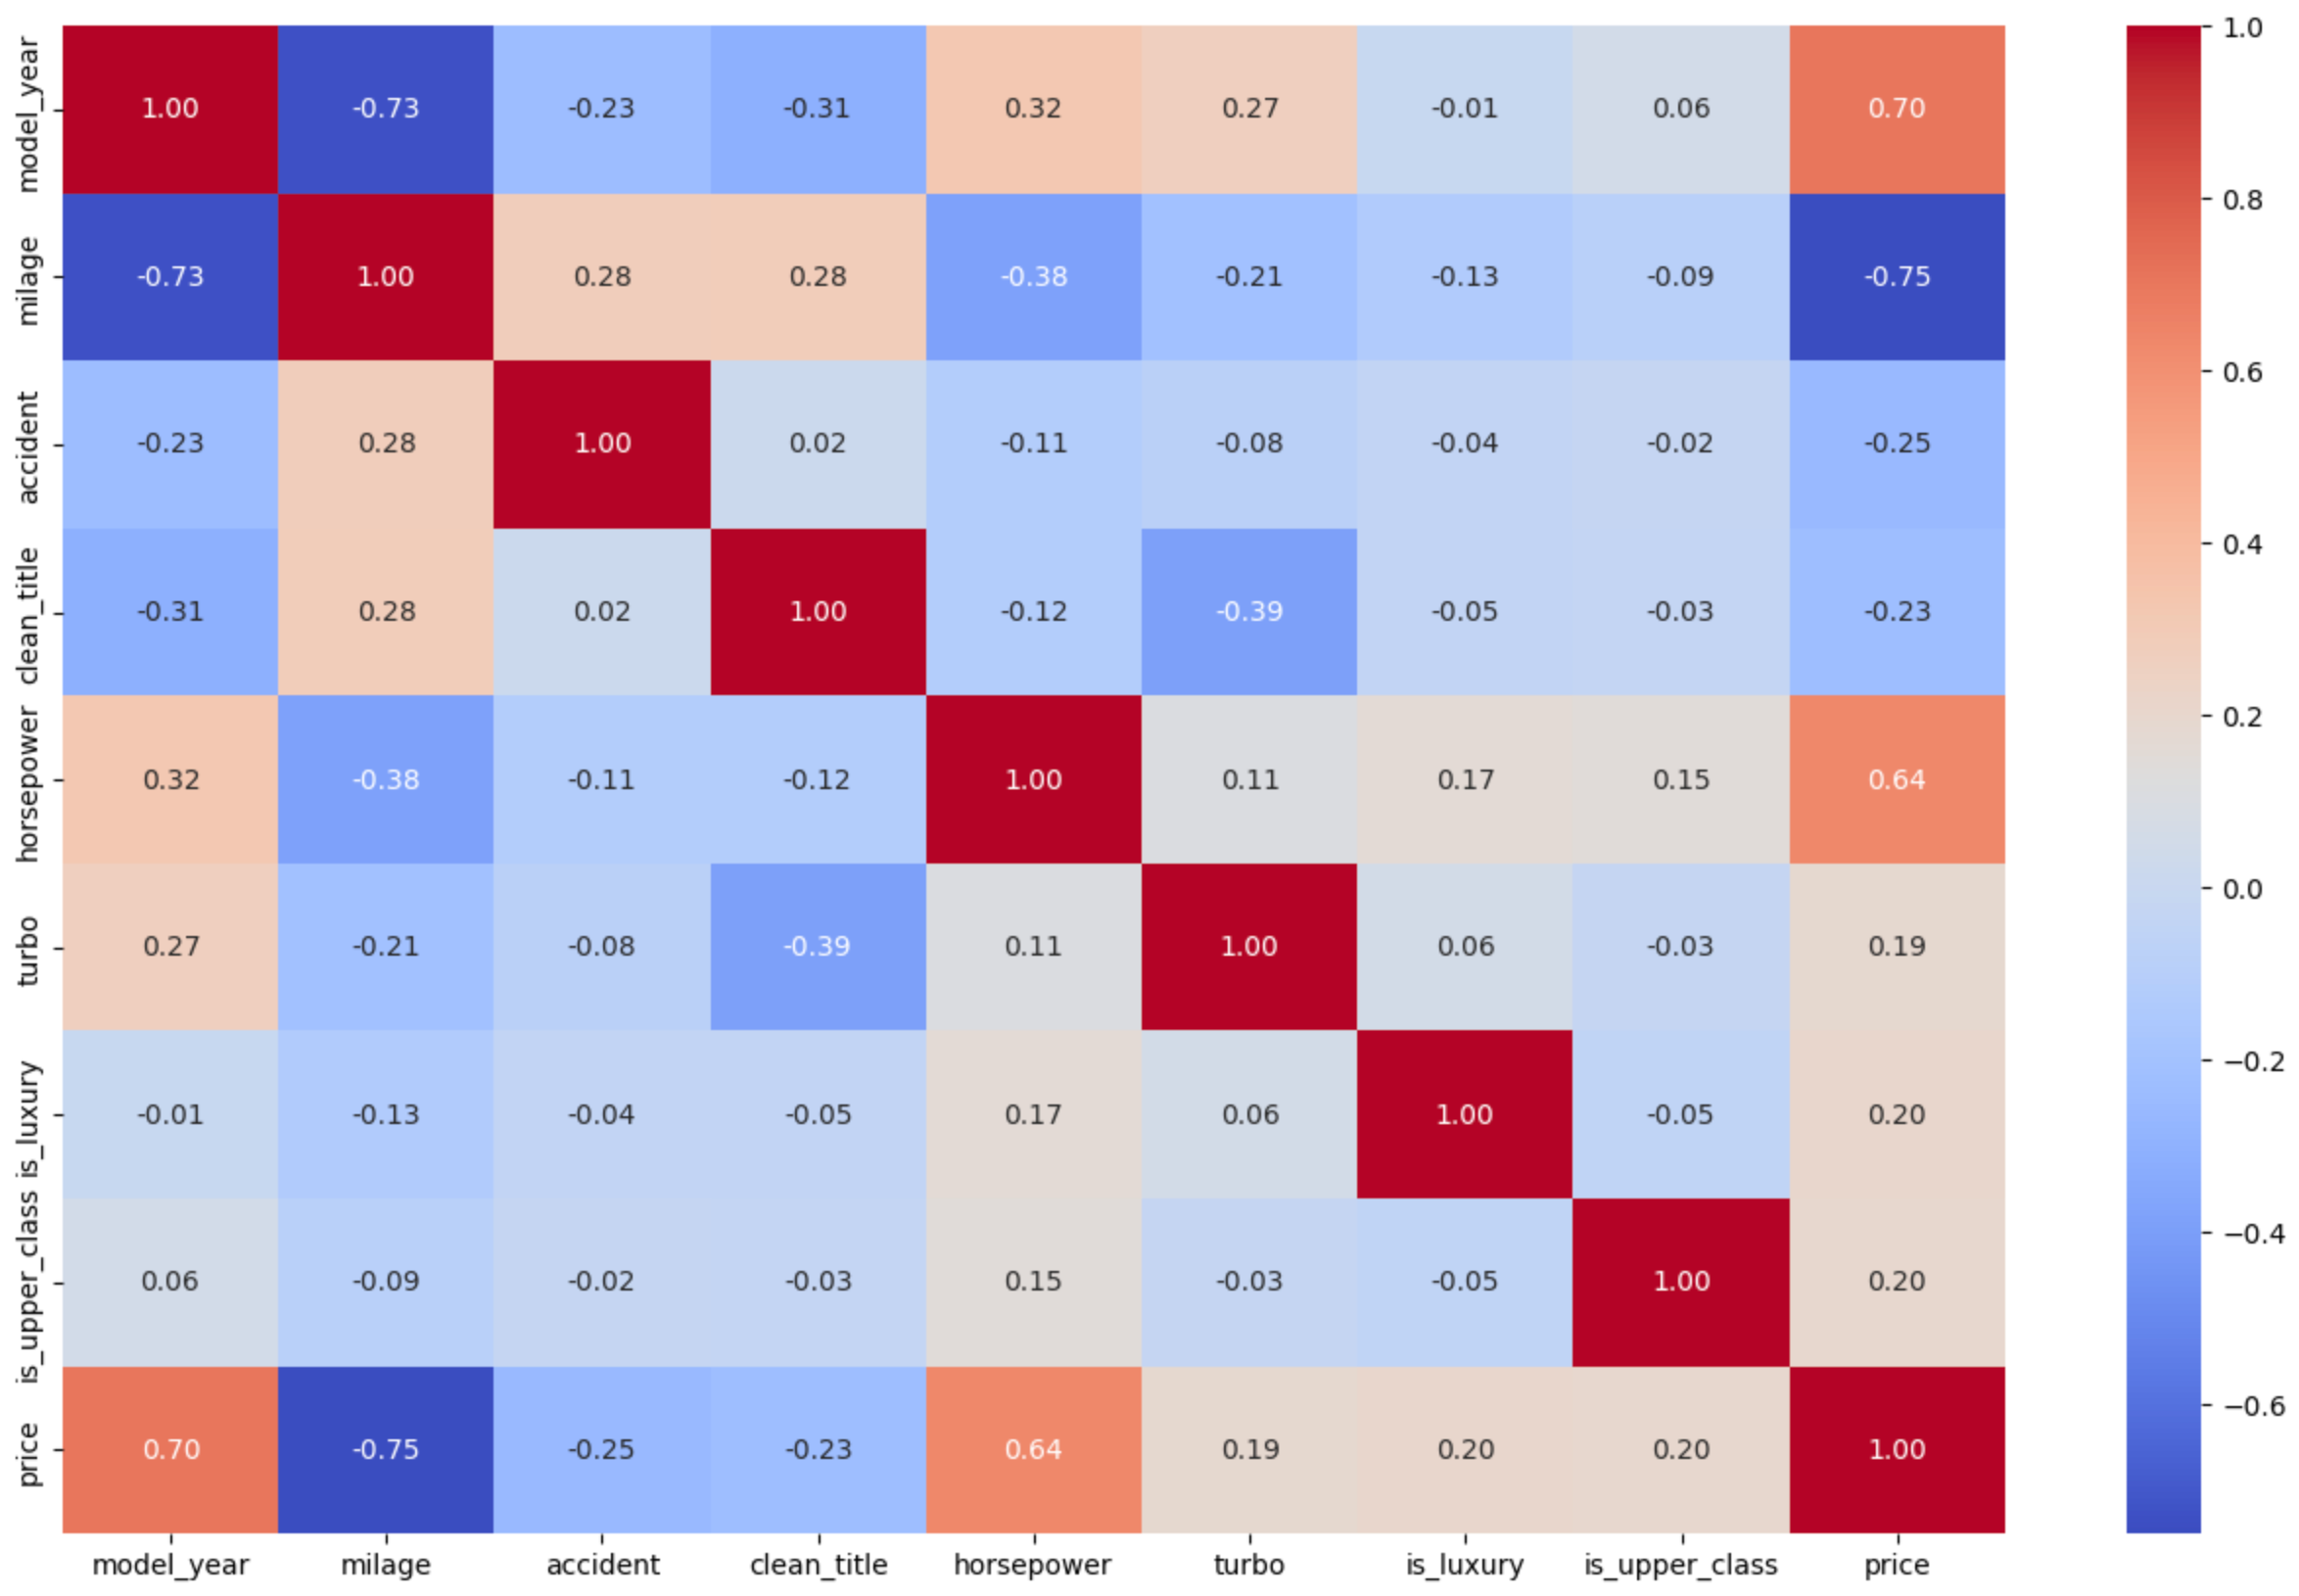
\includegraphics[width=\linewidth]{images/spearman_correlation.png}
	\centering
\end{wrapfigure}

The high negative correlation (-0.75) between~\textbf{\texttt{mileage}}~and~\textbf{\texttt{price}}~aligns with the intuitive understanding that higher mileage reduces a car's value, while the strong positive correlation (0.70) between~\textbf{\texttt{model\_year}}~and~\textbf{\texttt{price}}~reflects the higher value of newer cars. Notably,~\textbf{\texttt{mileage}}~and~\textbf{\texttt{model\_year}}~are themselves highly correlated (-0.73), as older cars typically have higher mileage. However, due to missing sale date information, these features were retained separately to avoid inaccuracies in modeling.

The Spearman correlation matrix provided essential insights for feature selection, emphasizing the predictive importance of mileage, model year, horsepower, and class-related depreciation. These findings laid the groundwork for further analyses, detailed in the following sections.

\section{Model Year and Price}
\label{sec:modelYearAndPrice}

The relationship between~\textbf{\texttt{model\_year}}~and~\textbf{\texttt{price}}~reveals a clear trend: older vehicles generally command lower prices, reflecting the depreciation associated with age. Newer vehicles retain higher market values due to technological advancements, improved efficiency, and perceived reliability. However, this trend is not uniform and is accompanied by notable exceptions and insights.

One prominent outlier is a~\textbf{Ford Bronco}~from an earlier model year, which retains a high value despite its age. This highlights the unique behavior of rare or collectible vehicles, whose values can appreciate due to scarcity, historical importance, and collector demand. Such anomalies underscore the need to account for market segmentation when analyzing price trends, as vintage cars do not follow typical depreciation models.

Price variance also differs significantly across model years. For newer vehicles (2020--2024), variance is high, driven by a mix of luxury cars, high-performance models, and electric vehicles. In contrast, older cars, especially those from before 2000, exhibit much lower price variance, reflecting their reduced functional value and the diminishing impact of brand and model differences. The convergence of prices for older cars suggests a more uniform valuation as vehicles age.

A box plot of~\textbf{\texttt{price}}~grouped by~\textbf{\texttt{model\_year}}~illustrates these patterns. Newer cars show a broader interquartile range, indicating greater diversity in pricing, while older vehicles display tighter price distributions. Median prices steadily decline with older model years, affirming the expected depreciation trend. The plot also highlights outliers, such as high-value vintage cars, which stand out above the general price range for older model years.

These findings align with the Spearman correlation analysis, where~\textbf{\texttt{model\_year}}~demonstrated a strong positive correlation (0.70) with~\textbf{\texttt{price}}. This emphasizes~\textbf{\texttt{model\_year}}~as a critical predictor in the dataset while underscoring the importance of recognizing exceptions, such as vintage vehicles. The combination of descriptive statistics and visualizations captures both the general depreciation trend and unique anomalies, providing a comprehensive understanding of this feature's impact.

\section{Milage and Price}
\label{sec:milageAndPrice}

The relationship between mileage and price follows an expected trend: as mileage increases, a car's value decreases. This negative correlation, identified in the Spearman correlation matrix (-0.75), reflects the perception that higher mileage indicates greater wear and tear, reducing a vehicle's market value and desirability. However, the impact of mileage on price varies significantly across vehicle classes.

\begin{figure}[h]
	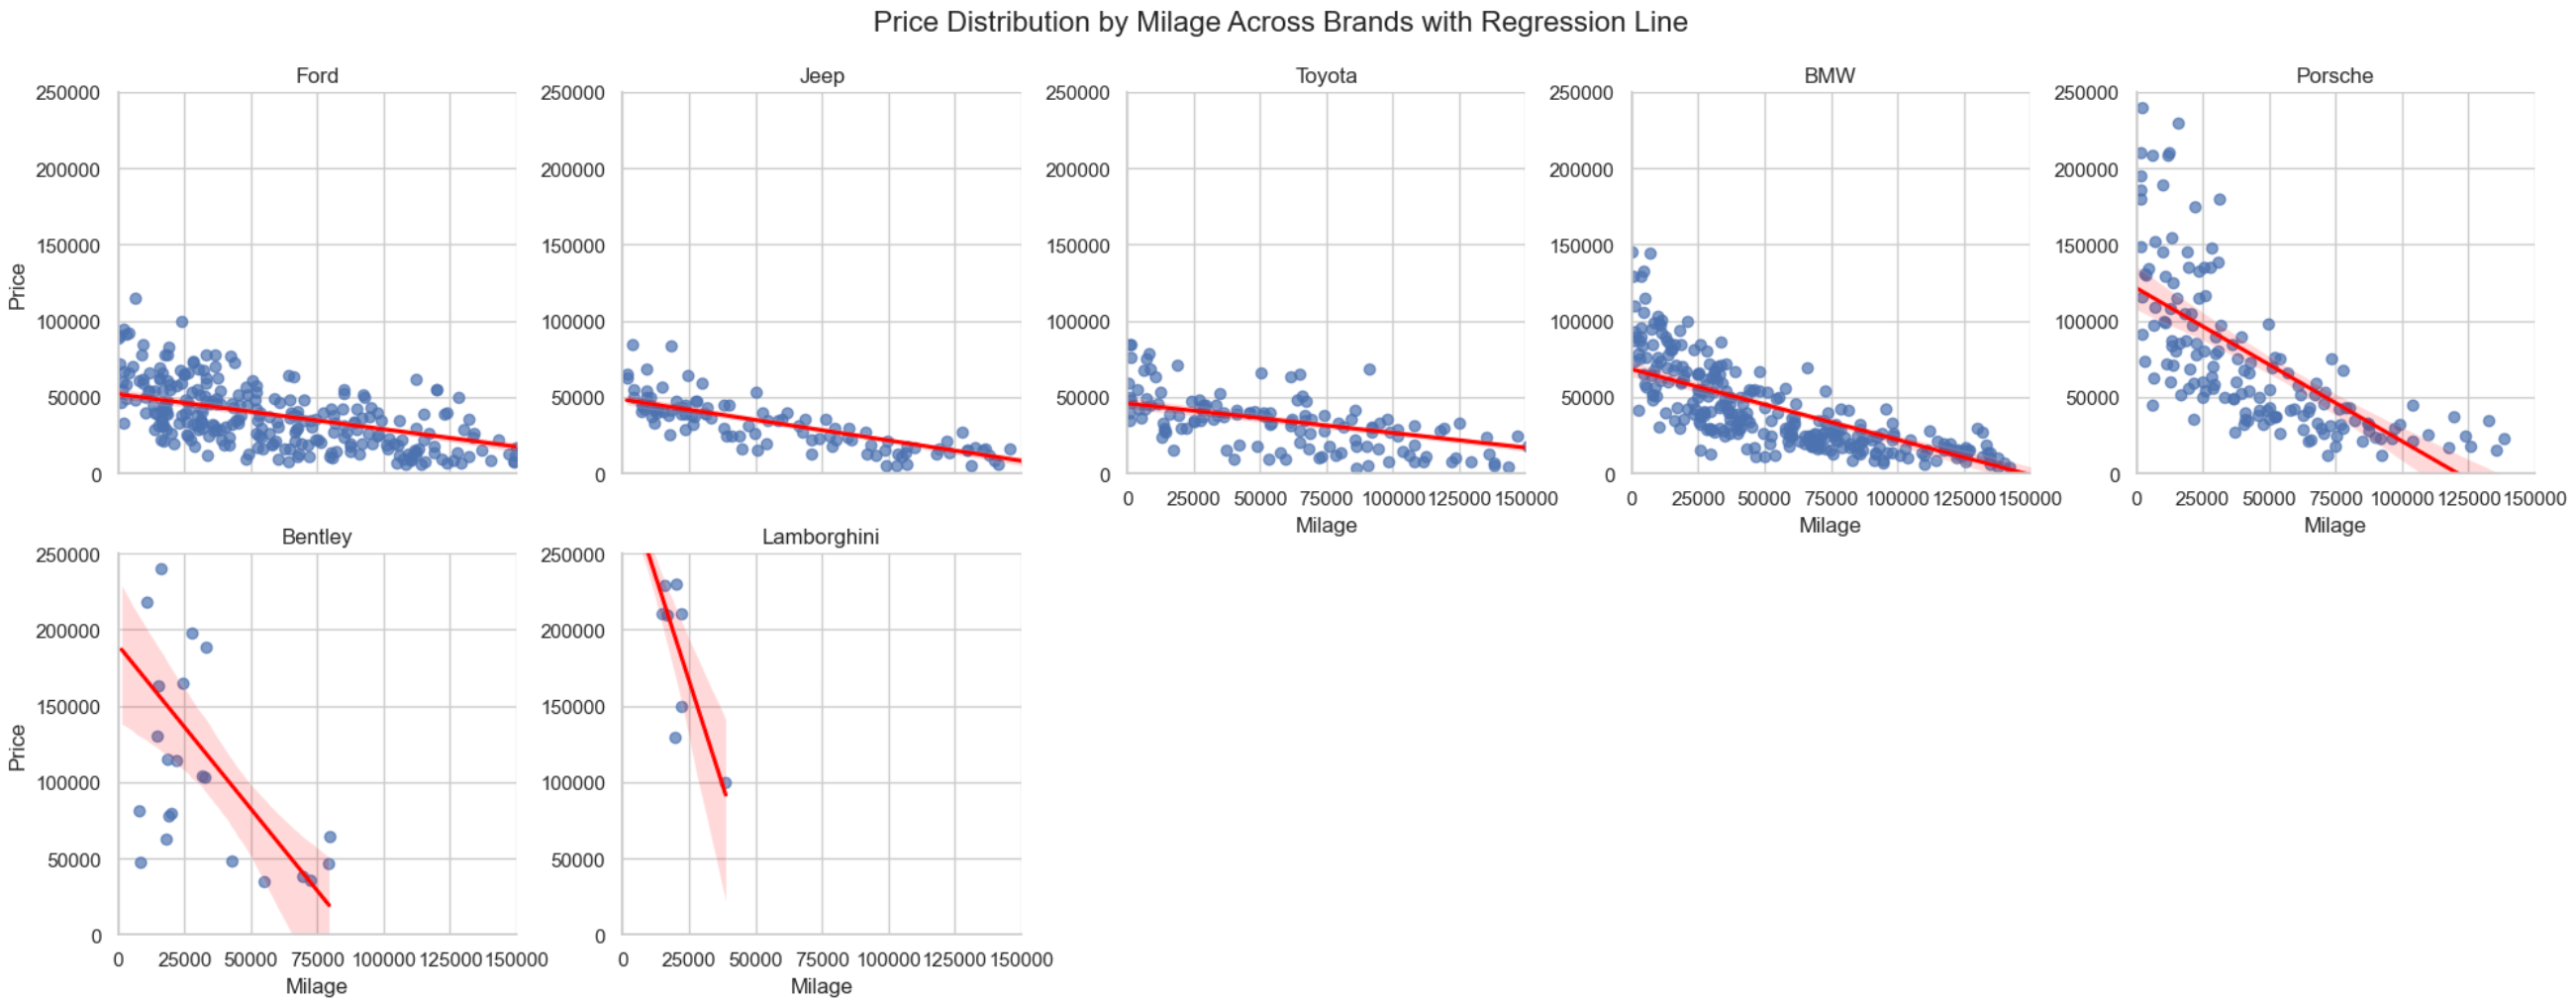
\includegraphics[width=\linewidth]{images/milage_price.png}
	\centering
\end{figure}

Luxury brands like Bentley and Lamborghini exhibit steep depreciation per mile compared to upper-class brands such as Porsche and standard brands like Toyota and BMW. In the luxury market, buyers presumably prioritize low mileage as a marker of exclusivity and pristine condition. Consequently, small increases in mileage can lead to substantial drops in value, with regression lines for Bentley and Lamborghini showing steep slopes. In contrast, upper-class brands like Porsche experience more moderate depreciation rates. While these cars retain elements of prestige, buyers are generally more accepting of moderate mileage, resulting in a less pronounced decline in value compared to luxury brands.

For standard brands like Toyota and BMW, the impact of mileage on price is the least severe. These vehicles are often valued for practicality and reliability, leading to slower and steadier depreciation rates. Their regression lines exhibit gentler slopes, highlighting their resilience to value loss with increased mileage.

At lower mileage levels, luxury cars display greater price variability due to differences in model configurations, rarity, and demand. For instance, Lamborghinis and Bentleys at similar mileage levels may have vastly different valuations based on trim levels or limited-edition status. In contrast, standard brands like Toyota and BMW exhibit tighter price distributions at low mileage, reflecting a more uniform valuation process.

These findings underscore the importance of vehicle class in determining how mileage affects price. Recognizing the varying depreciation rates across classes enables predictive models to better capture real-world pricing dynamics. This nuanced approach enhances model accuracy by incorporating the interplay of mileage, vehicle class, and market expectations.

\section{Horsepower and Price}
\label{sec:horsepowerAndPrice}

The relationship between horsepower and price shows a clear positive correlation: vehicles with higher horsepower tend to command higher prices. This aligns with market expectations, as greater horsepower is associated with enhanced performance, advanced engineering, and premium vehicle categories, which justify higher price points. However, this relationship is not strictly linear and exhibits notable variability.

For vehicles with horsepower between 200 and 300, prices range widely from below \$20,000 to over \$60,000. This spread indicates that horsepower alone does not determine price; other factors, such as brand, model, mileage, and additional features, significantly influence market value. Additionally, most vehicles fall within the 100--300 horsepower range, reflecting the dominance of standard consumer vehicles in the dataset. In contrast, cars with over 400 horsepower are rarer and typically represent luxury or high-performance models with premium price tags.

Outliers in the upper-right portion of the scatter plot---vehicles with extreme horsepower and price---highlight niche categories such as sports cars or limited-edition models. These outliers emphasize the dataset's heterogeneity and the need to account for market segmentation in predictive modeling.

Horsepower values were not always available in the dataset and were imputed using related features such as cubic capacity and cylinder count. This imputation leveraged strong correlations between these attributes to estimate missing values. However, imputed values may introduce some uncertainty, particularly for vehicles where cubic capacity or cylinder count alone cannot fully capture performance characteristics.

In summary, while higher horsepower correlates with higher prices, significant variability exists within this trend, influenced by additional factors such as market demand and vehicle class. These insights highlight the importance of incorporating horsepower into predictive models while accounting for its interactions with other features.

\chapter{Models}
\label{cha:models}

To evaluate the predictive capabilities of machine learning models, we tested four algorithms: Linear Regression, Polynomial Regression, Random Forest, and XGBoost on our dataset. Additionally, we assessed a model trained on synthetic data using XGBoost to explore the impact of synthetic data augmentation. The median car price and the Linear Regression model served as our baselines due to their simplicity and interpretability, providing a reference for comparing more complex approaches.

Our modeling process followed a standardized approach inspired by coursework methodology. For each model, we defined a parameter grid (\textbf{\texttt{param\_grid}}) of various parameter combinations. A five-fold cross-validation was performed for each, normalizing train and test data independently. Polynomial Regression included polynomial transformations before normalization to capture non-linear patterns. After evaluating all parameter combinations, the best-performing configuration was used to train the final model on the entire training set, ensuring optimal performance.

The median car price as a baseline shows an MAE of 17,794.41, MAPE of 91.59\%, and  R² score of 0 (baseline) on the test set. Linear Regression achieved an MAE of 14,471.85, a MAPE of 50.26\%, and an R² score of 0.5639, serving as a benchmark for more complex models. The simplicity of median and linear regression made them easy to interpret, but their inability to capture (non-linear) relationships limited predictive performance. Polynomial Regression improved on these results, achieving an MAE of 12,273.10, a MAPE of 36.14\%, and an R² score of 0.6620, demonstrating its ability to model complex relationships. However, the model required careful tuning to prevent overfitting, particularly with higher-degree polynomials.

The Random Forest Regressor further enhanced performance, with an MAE of 11,384.63, a MAPE of 33.70\%, and an R² score of 0.7008. Its ensemble approach, averaging predictions from multiple decision trees, provided robustness against noise and outliers. Key hyperparameters, including 50 estimators (\textbf{\texttt{n\_estimators}}), a maximum depth of 10 (\textbf{\texttt{max\_depth}}), and a minimum of 2 samples to split a node (\textbf{\texttt{min\_samples\_split}}), balanced complexity and generalization. Random Forest excelled in handling mixed data types and offered insights into feature importance, making it a valuable addition to the analysis.

XGBoost emerged as the best-performing model on the original dataset, with an MAE of 11,314.81, a MAPE of 33.33\%, and an R² score of 0.7039. The gradient boosting framework allowed it to iteratively refine predictions, capturing subtle data patterns overlooked by simpler models. The optimal configuration included 100 estimators (\textbf{\texttt{n\_estimators}}), a maximum depth of 5 (\textbf{\texttt{max\_depth}}), and a learning rate of 0.05 (\textbf{\texttt{learning\_rate}}), among other parameters. These settings balanced precision and generalization while avoiding overfitting. XGBoost's ability to handle missing data and complex feature interactions contributed to its superior accuracy, making it the most effective model in our analysis.

To test synthetic data augmentation, we trained XGBoost on a dataset with 100,000 synthetic entries. While XGBoost was chosen for consistency, its performance degraded significantly, with an MAE of 9,910.14, a MAPE of 42.03\%, and an R² score of 0.6135. This decline highlights challenges with synthetic data, such as inconsistencies and noise introduced during generation, which obscured meaningful patterns and hindered generalization.

This analysis underscores the progressive improvements achieved by increasingly sophisticated models, starting with Linear Regression and culminating in XGBoost. Parameter tuning and cross-validation maximized each model's performance. The inclusion of synthetic data revealed the importance of data quality over quantity, emphasizing that effective preprocessing and careful model selection are essential for achieving optimal predictive accuracy.

\chapter{Results and Evaluation}
\label{cha:resultsAndEvaluation}

\begin{wrapfigure}{r}{0.5\textwidth}
	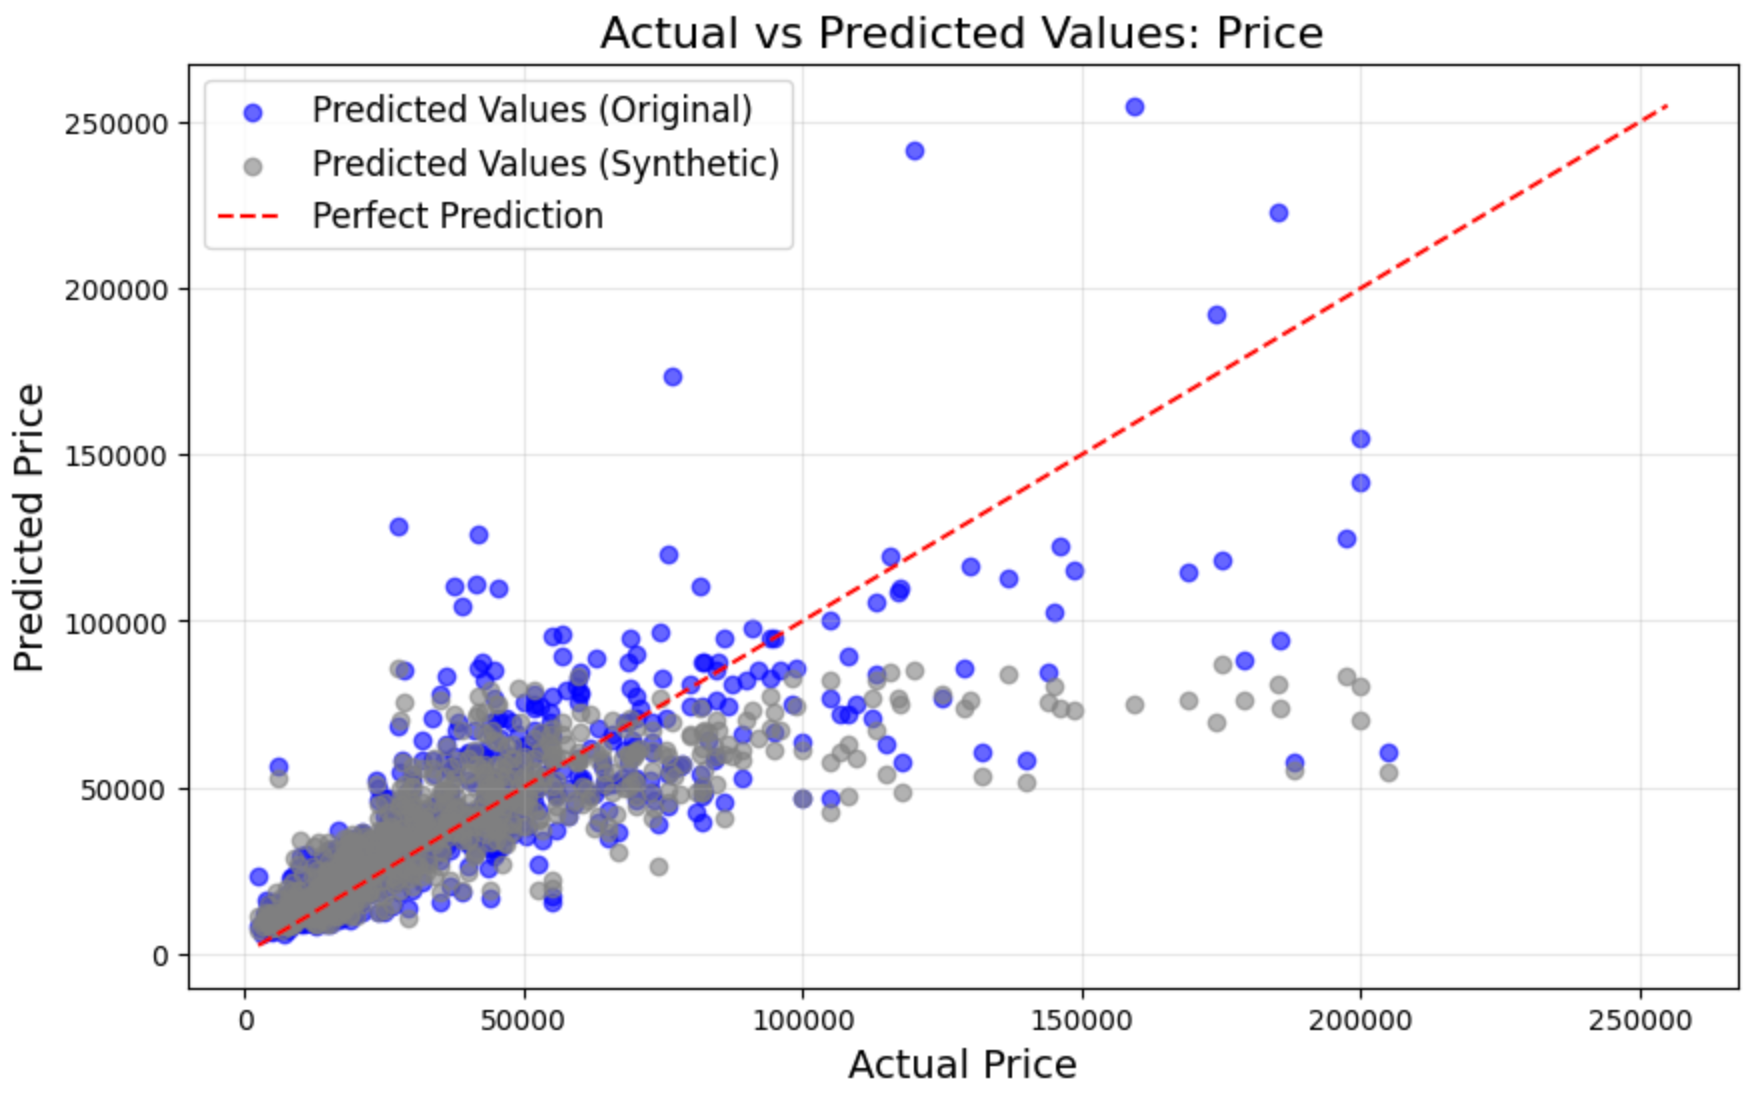
\includegraphics[width=\linewidth]{images/xgb_results_mixed.png}
	\centering
\end{wrapfigure}

The evaluation began with a baseline comparison using Linear Regression, which achieved an MAE of 13,632.41, a MAPE of 50.05\%, and an R² score of 0.6253. Although modest in performance, it provided a valuable benchmark for assessing the improvements offered by more complex models.

XGBoost emerged as the best-performing model on the original dataset, achieving an MAE of 11,314.81, a MAPE of 33.33\%, and an R² score of 0.7039. Its gradient boosting framework captured subtle patterns and feature interactions, slightly outperforming Random Forest (MAE: 11,384.63, R²: 0.7008) and highlighting the advantages of XGBoost's iterative optimization and regularization techniques.

Models trained on the original dataset consistently outperformed those using synthetic data. For example, XGBoost trained on synthetic data achieved an MAE of 9,910.14, a MAPE of 42.03\%, and an R² score of 0.6135, overall lower than its performance on the original dataset. Despite the synthetic dataset's larger size (100,000 entries vs.~3,200), poor quality, including mixed-up car configurations, outliers, and unrealistic combinations, likely contributed to this disparity. The differing distributions between synthetic and original data further amplified the performance gap, especially since evaluation was conducted on a subset of the original dataset.

Finally, our XGBoost model trained on the original dataset achieved a Root Mean Squared Error (RMSE) of 19,936.60 far surpassing the competition's median RMSE of 71,900 on Kaggle. This significant performance gap prompted thorough checks for potential information leakage, but no evidence of such issues was found. The results reflect robust preprocessing and effective modeling strategies. Further exploration of this disparity is provided in the critical reflection section.

\chapter{Critical Reflection}
\label{cha:criticalReflection}

This study offers valuable insights into the potential impact of synthetic data on predictive modeling for car retail prices but is subject to several limitations affecting the validity and generalizability of its findings.

The dataset lacks critical features, such as interior specifications, reasons for sale, ownership history, or overall condition, which are essential for capturing nuanced determinants of pricing. Without these variables, the model's predictive power is inherently constrained. Additionally, inconsistent model name representations introduced significant noise. For instance, variations in labeling a ``VW Golf'' hindered the model's ability to extract meaningful distinctions. Given the dataset's small size, this issue further limited learning, forcing the omission of the model name feature, despite its relevance in determining price.

The ambiguity surrounding price determination further complicates the analysis. It is unclear whether prices were set by owners, dealerships, or other entities. We assumed owner-set prices, which could explain anomalies like a Bentley priced below \$50,000 with fewer than 8,000 miles, likely reflecting a quick-sale priority. However, without clarity on price-setting methods, this assumption introduces uncertainty, potentially impacting the model's generalizability.

While the dataset includes the~\textbf{model year}, the absence of~\textbf{sale dates}~prevents accurate calculation of vehicle age at the time of sale. This missing data forced us to retain~\textbf{model year}~and~\textbf{mileage}~as separate features, despite their high correlation, avoiding speculative inferences but potentially missing more informative insights.

The dataset's origin from a Kaggle competition allowed for performance benchmarking. Our model achieved an RMSE of 16,457, significantly outperforming the competition's median of approximately 71,900. While this highlights the robustness of our approach, the discrepancy invites scrutiny. Despite thorough checks, no evidence of information leakage was found. Our decision to exclude sales above \$1 million likely reduced noise, potentially explaining the performance gap if other groups included these outliers. Alternatively, the discrepancy could result from random factors, such as favorable imputations or test set splits.

These findings emphasize the importance of high-quality, well-documented data. Improved datasets with richer attributes, consistent formatting, and clear price-setting mechanisms would enable more robust modeling and enhance the applicability of machine learning techniques in car price prediction.

\backmatter

\bibliography{references}
\label{bibliography}

\chapter{Ehrenwörtliche Erklärung}
\label{cha:ehrenwoertlicheErklaerung}

Ich versichere, dass ich die beiliegende Bachelor-, Master-, Seminar-, oder
Projektarbeit ohne Hilfe Dritter und ohne Benutzung anderer als der angegebenen
Quellen und in der untenstehenden Tabelle angegebenen Hilfsmittel angefertigt
und die den benutzten Quellen wörtlich oder inhaltlich entnommenen Stellen als
solche kenntlich gemacht habe. Diese Arbeit hat in gleicher oder ähnlicher Form
noch keiner Prüfungsbehörde vorgelegen. Ich bin mir bewusst, dass eine falsche
Erklärung rechtliche Folgen haben wird.

% Declare below which AI tools you used in the process of writing your work,
% including text, image, code, and data generation. If you used a tool for a
% purpose not included in the list yet, add it to the list.
\begin{center}
  \textbf{Declaration of Used AI Tools} \\[.3em]
  \begin{tabularx}{\textwidth}{lXlc}
    \toprule
    Tool & Purpose & Where? & Useful? \\
    \midrule
    ChatGPT & Rephrasing & Throughout & ++ \\
    Github Copilot & Code Completion & Jupiter Notebook & ++ \\
    DeepL & Translation & Throughout & ++ \\
    \bottomrule
  \end{tabularx}
\end{center}

\vspace{1.8cm}
\noindent Unterschriften\\
\noindent Mannheim, den 08.~Dezember 2024 \hfill

\end{document}
